\documentclass[12pt]{article}

\usepackage[a4paper, margin=2.5cm]{geometry}
\usepackage{graphicx}
\usepackage{fontenc}
\usepackage{inputenc}
\usepackage{setspace}
\usepackage{hyperref}
\usepackage{setspace}
\usepackage{booktabs}
\usepackage{caption}
\usepackage{subcaption}
\usepackage{amsmath}
\usepackage{hyperref}

\begin{document}

\begin{titlepage}
    \centering

    % University logo
    
\includegraphics[width=0.45\textwidth]{images/ozu_logo.png}\\[3cm]

    % Course
    {\large \textbf{EE 350 -- Electronics II}}\\[1cm]

    % Semester
    {\large \textbf{Spring 2025/26}}\\[1cm]

    % Lab number
    {\large \textbf{LAB 2}}\\[1cm]

    % Lab title
    {\large \textbf{DIFFERENTIAL AMPLIFIERS}}\\[5cm]

    % Submission info
    \begin{center}
        {\normalsize \textbf{Submitted by:} Ömer Faruk AVCI}\\[0.4cm]
        {\normalsize \textbf{Student ID:} S034113}\\[0.4cm]
        {\normalsize \textbf{Date of Submission:} 14.04.2026}
    \end{center}

\end{titlepage}


% Introduction
\section*{Introduction}
In this laboratory session, we are required to build and analyze a differential amplifier implemented with BJTs using a CA3146 transistor array. After constructing the circuit, we will examine its behavior under different conditions, including common-mode, large-signal transfer characteristics, and small-signal gain. While differential amplifiers are used in many electronics applications, for example, in sensor signal conditioning, audio amplification, and communication circuits, the lab will help in grasping the fundamental operating principles and gain characteristics of these circuits under various signal conditions.

\newpage
% Experiments 
\section*{Experiments}
\subsection*{Task 1: Common Mode Analysis}

While the calculated resistor value in Prelab for $R_c$ was 2500 ohms, 2.2k ohm resistors were used in the actual circuit due to the unavailability of 2.5k ohm resistors. The given circuit was built on the breadboard using CA3146. The constructed circuit can be seen as follows:

\begin{figure}[h]
        \centering
        
\includegraphics[width=0.7\linewidth]{images/task1_circuit.png}
    \caption{Breadboard Implementation of the Circuit}
\end{figure}

After constructing the circuit and turning on the power supplies, a multimeter is utilized to measure the voltage difference between pins 1 and 5, which corresponds to the outputs of the differential amplifier on the CA3146 IC. Since the input was a 5V DC source, as expected, the multimeter measured 0.02V, as shown in Figure 2.

\begin{figure}[h]
        \centering
        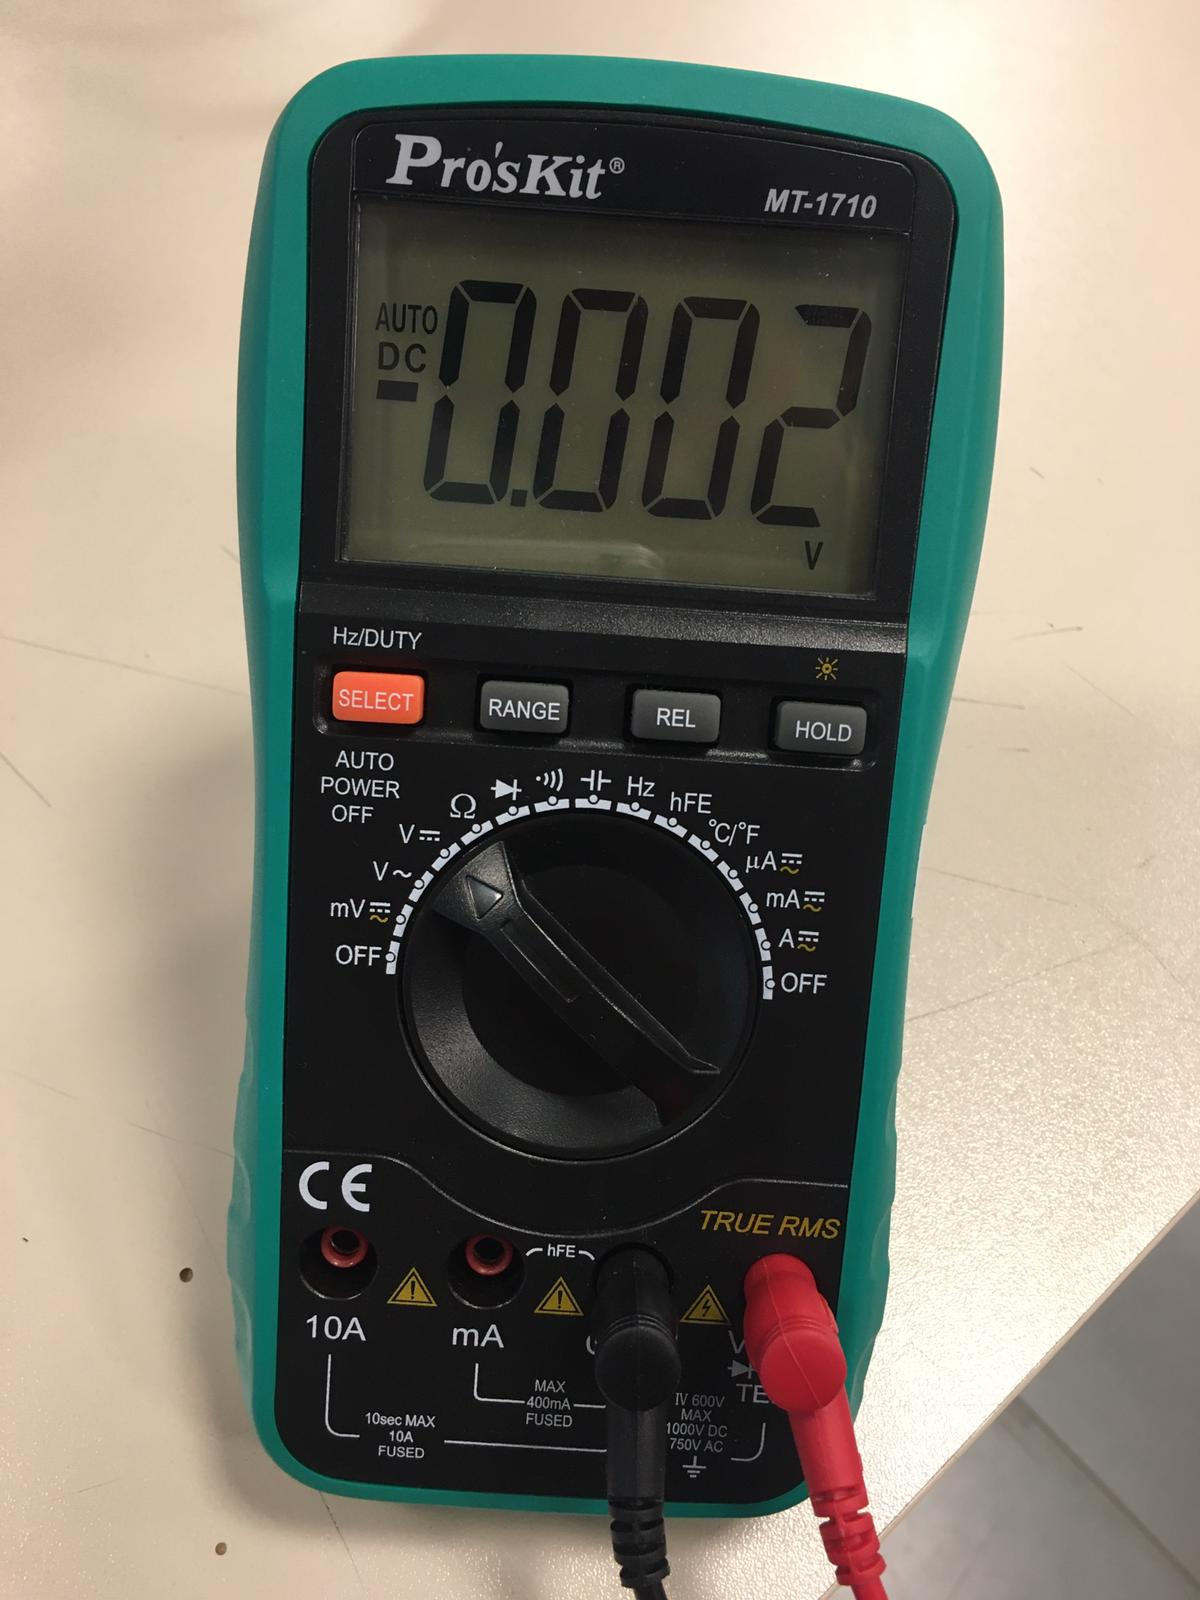
\includegraphics[width=0.33\linewidth]{images/task1_measurement.png}
    \caption{Multimeter Measurement }
\end{figure}

Ideally, a common-mode input should have resulted in a 0V differential output. The measured 20 mV offset is expected and is primarily due to practical non-idealities, such as tolerance variations in the physical 2.2 k ohm resistors and internal mismatches between transistors within the IC array.

\newpage

\subsection*{Task 2: Large Signal Analysis}

The circuit built in Task 1 was retained for Task 2, which is about large-signal analysis. The input signals were changed from a 5V DC common-mode source to a differential AC source, specifically 150 mV peak-to-peak triangular waves with a 180-degree phase shift. Using the two probes of the oscilloscope, one of the inputs and the outputs of the circuit were monitored. 

\subsubsection*{Time Domain Analysis}

The input and output waveforms were initially observed in the time domain, as shown in Fİgure 3. Channel 1 displays the triangular input signal, measured at 148.0 mV peak-to-peak and 1.00 kHz. Channel 2 displays the corresponding single-ended output signal from the differential amplifier, measured at 4.40 V peak-to-peak. 

\begin{figure}[h]
        \centering
        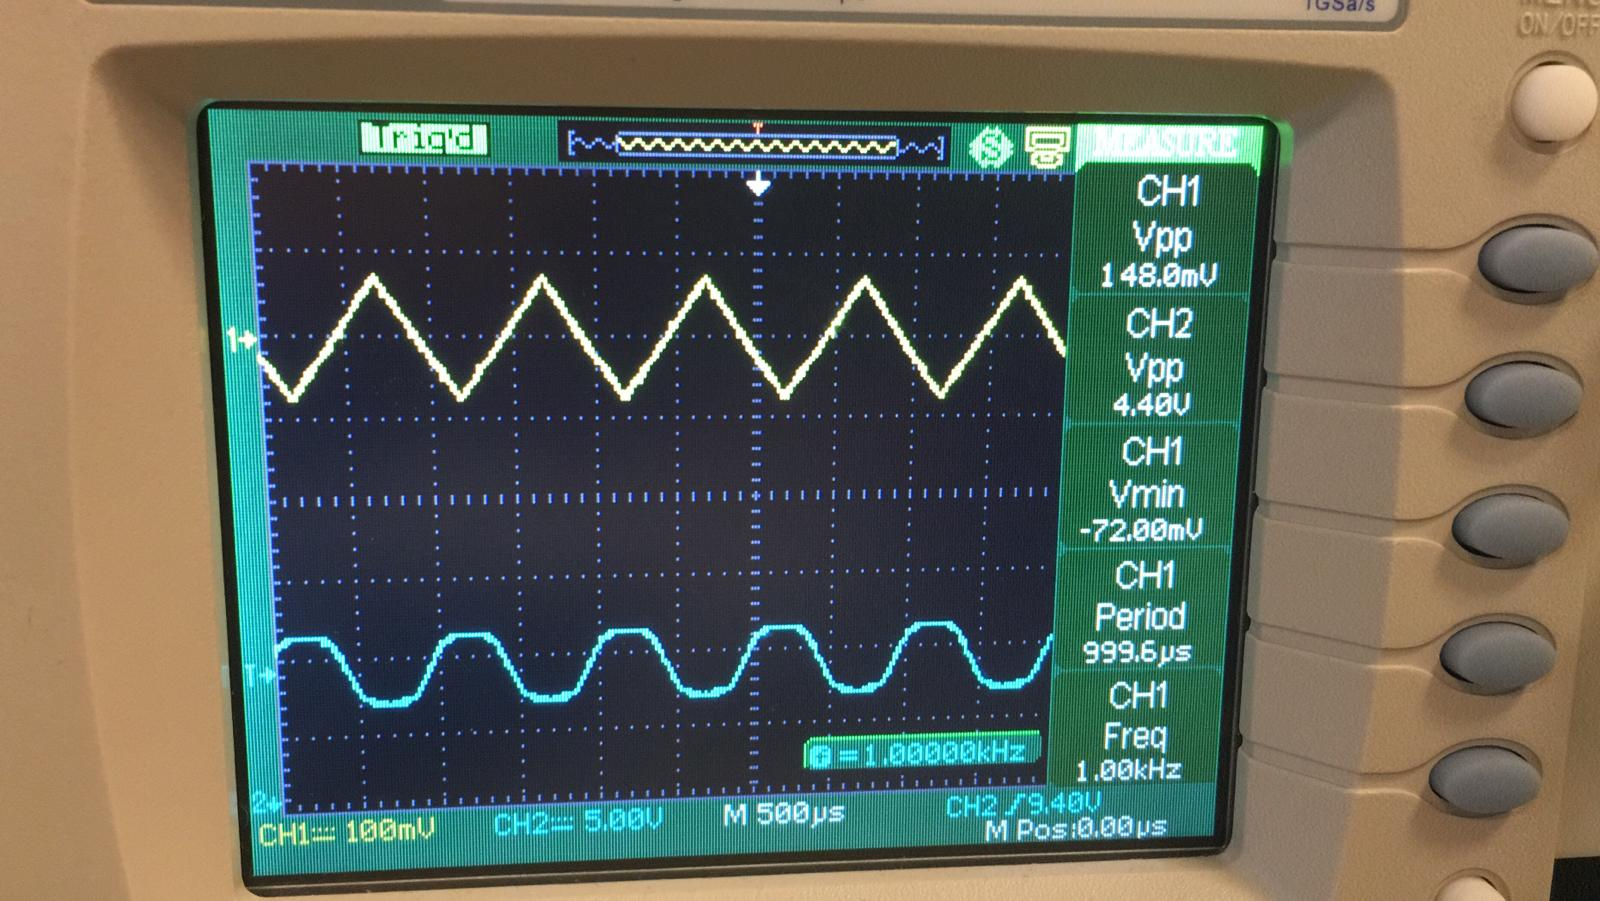
\includegraphics[width=0.75\linewidth]{images/task2_graph.png}
    \caption{Input and Output Waveform for Large Signal}
\end{figure}

The flattening observed in the output waveform is due to transistor saturation and cutoff. When the differential input voltage is large (±150mV creating 300mV differential), the amplifier attempts to produce an output beyond the ±12V supply rails. This causes one transistor to saturate while the other enters cutoff, resulting in the clipped/flattened regions of the transfer characteristic. This demonstrates the limited linear range of the differential amplifier for large signal operation

\subsubsection*{X-Y Domain Analysis}

When the oscilloscope is switched to X-Y mode, as shown in Figure 4 , the time variable is eliminated. This configuration plots the single-ended output voltage directly against the input voltage, revealing the large-signal voltage transfer characteristic (VTC) of the differential amplifier. The resulting transfer curve exhibits a distinct "S" shape, characteristic of the BJT differential pair's hyperbolic tangent profile. The negative slope in the center indicates an inverting relationship between the specific input and output nodes being probed.

\begin{figure}
        \centering
        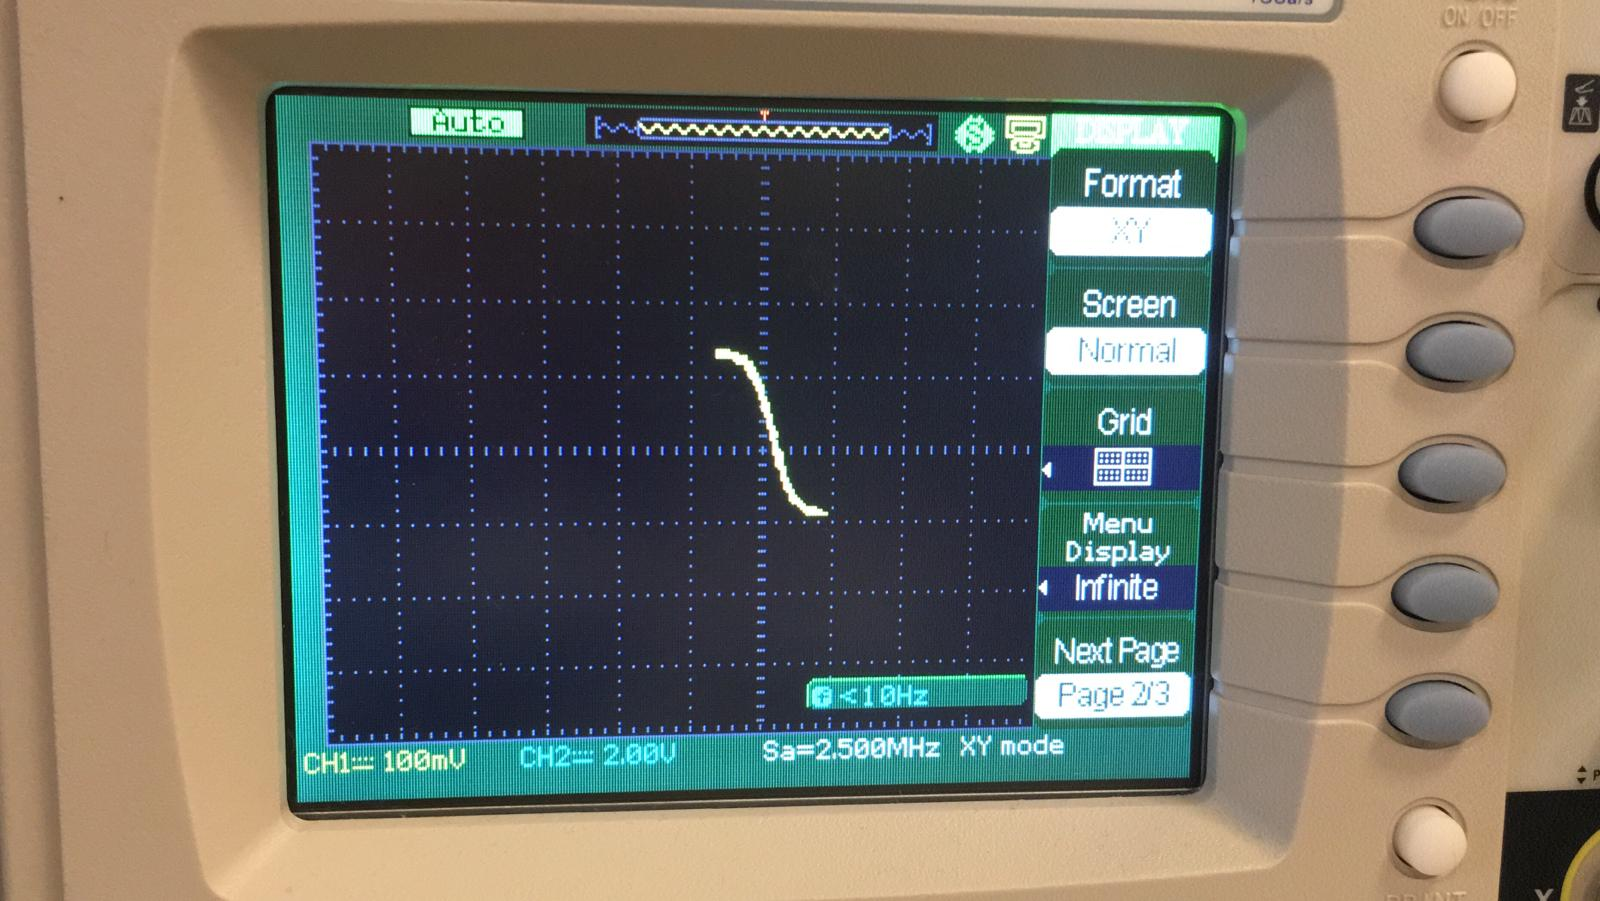
\includegraphics[width=0.75\linewidth]{images/task2_xy.png}
    \caption{X-Y Mode Waveform}
\end{figure}

\newpage

\subsection*{Task 3: Small Signal Analysis}

The large signal inputs from Task 2 were replaced with small-signal 1kHz differential 10 mV peak-to-peak sine wave with a 180-degree phase shift between the channels. The output waveform is as follows:

\begin{figure}[h]
        \centering
        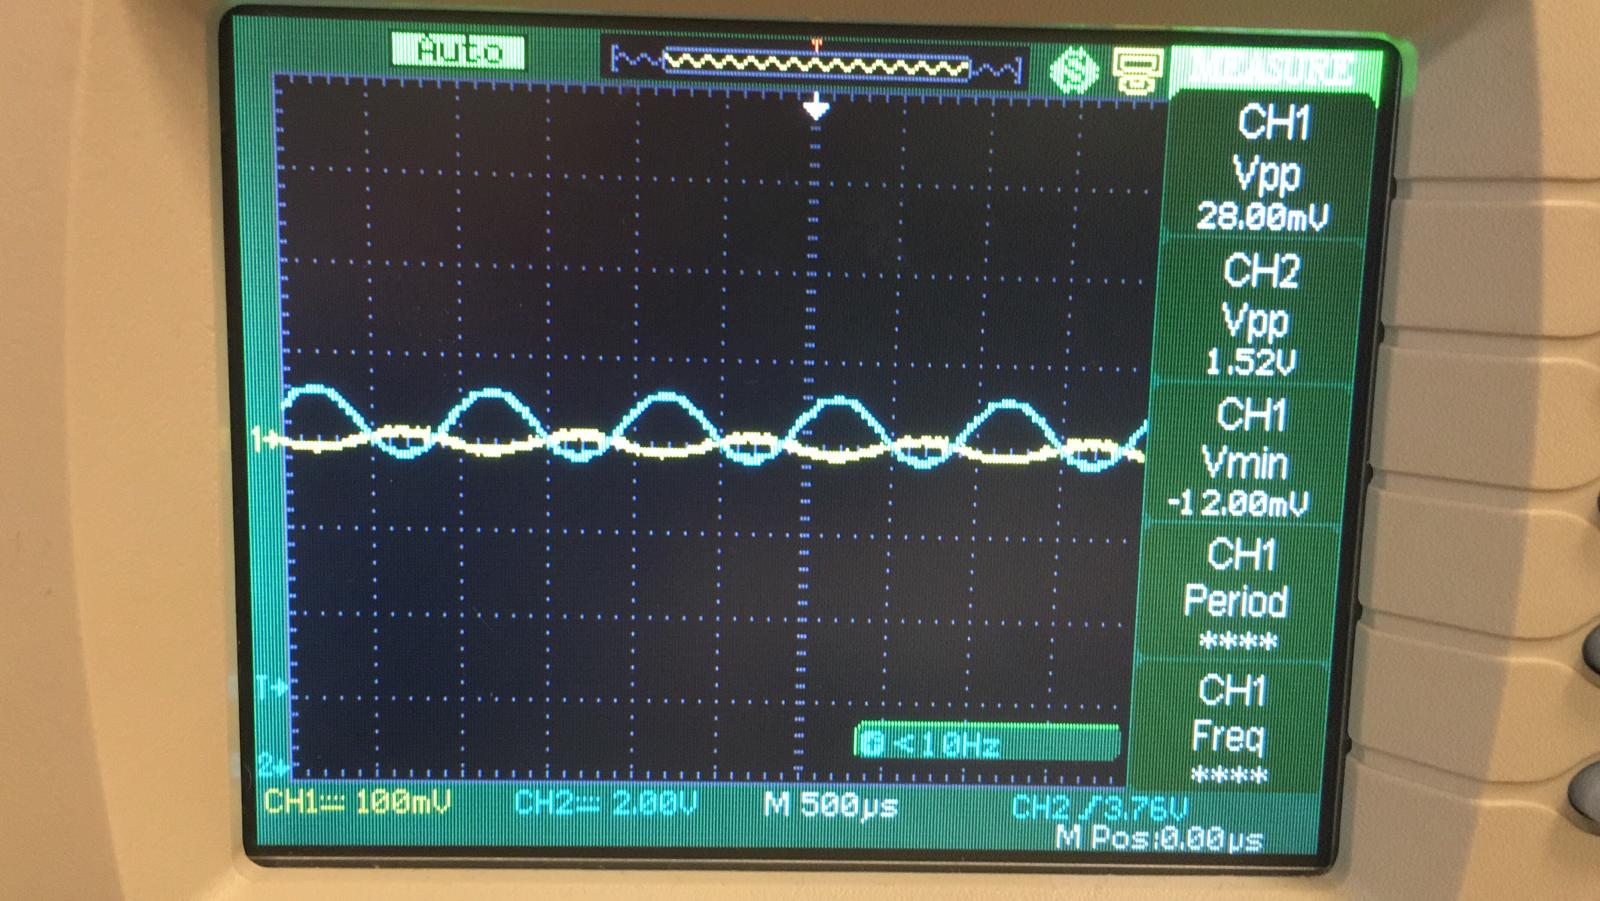
\includegraphics[width=0.75\linewidth]{images/task3_graph.png}
    \caption{Input and Output Waveform for Small Signal}
\end{figure}

As shown in Figure 5, Channel 1 monitored one of the single-ended inputs, recording a peak-to-peak voltage ($V_{in-pp}$) of 28.00 mV. Channel 2 monitored the corresponding single-ended output at the collector, recording a peak-to-peak voltage ($V_{out-pp}$) of 1.52 V. The waveforms demonstrate clear linear amplification without the saturation or clipping distortion observed during the large-signal analysis.

\textbf{Gain Calculation:} 

Using the measured peak-to-peak values, the practical voltage gain ($A_v$) of the amplifier can be calculated as follows:

$$A_v = \frac{V_{out-pp}}{V_{in-pp}} = \frac{1.52 \text{ V}}{0.028 \text{ V}} \approx 54.3 \text{ V/V}$$

While the targeted gain was 100, the circuit failed to meet with this requirement. The attenuation was expected but the reason for that much difference can be as: 

\begin{itemize}
    \item Input Signal Amplitude: The actual 28 mV peak-to-peak input (rather than the 10 mV target) pushes the transistors slightly out of their ideal linear region, reducing the effective transconductance.
    \item Component Substitution: Using 2.2 k ohm resistors instead of the calculated 2.5 k ohms directly lowers the gain, as voltage gain is directly proportional to the collector resistance.
    \item Transistor Non-Idealities: Real transistors in the CA3146 array have internal parasitic elements, such as finite output resistance and internal emitter resistance, which lower the overall gain compared to ideal theoretical models.
\end{itemize}

\section*{Conclusion}

In this laboratory, a BJT differential amplifier was constructed and evaluated using the CA3146 transistor array. The experiment successfully demonstrated the circuit's behavior across three distinct operating conditions:

\begin{itemize}
    \item \textbf{Common-Mode Rejection:} Applying a common 5 V DC input yielded a minimal 20 mV differential output. This verified the noise-rejection capability of the differential pair, with the slight offset primarily stemming from component tolerances and minor internal transistor mismatches.
    
    \item \textbf{Large-Signal Nonlinearity:} Utilizing a 150 mV peak-to-peak input drove the transistors into saturation and cutoff, visibly flattening the time-domain output. The X-Y mode observation successfully captured the signature hyperbolic tangent ("S-curve") voltage transfer characteristic of the BJT pair.
    
    \item \textbf{Small-Signal Amplification:} Under linear operation, the measured differential voltage gain was approximately 54.3 V/V. While lower than the targeted preliminary design gain of 100, the discrepancy was analytically justified by the substitution of 2.2 k$\Omega$ collector resistors, a larger-than-ideal input amplitude (28 mV), and intrinsic transistor parasitics.
\end{itemize}

Overall, the experiment provided a practical verification of both the linear amplification capabilities and the inherent nonlinear limitations of BJT differential amplifiers.
\end{document}